% 
\chapter{Análise e desenho da solução} % Main chapter title
\label{chap:ADS} % For referencing the chapter elsewhere, use Chapter~\ref{ADS}

O capítulo que se segue tem o principal objetivo de apresentar as diferentes fases ligadas ao processo de análise e desenho da solução. Inicia-se com a contextualização do domínio do problema, suportada por um modelo de domínio e por uma tabela de termos. Procede-se à especificação dos requisitos funcionais e não funcionais, antecedendo a identificação dos atores e dos casos de uso. Por último, descreve-se o desenho da solução, evidenciando os principais componentes e a arquitetura da aplicação.


%-------------------------------------------------------------------------------

\section{Domínio do problema} 
\label{sec:DP} 

Caracteriza-se o contexto operacional da plataforma \textbf{OnlyYes} e o núcleo do problema a resolver descrito na secção \ref{Problema}.

Esta secção estabelece o vocabulário comum e as relações conceptuais que suportam o desenho e a implementação da solução, e o modelo que caracteriza as regras de negocio.

\subsection{Glossário do Domínio}

O glossário acrescenta significado ao domínio, pois contêm termos fundamentais para clarificar retirar ambiguidades.

A Tabela~\ref{tab:glossario-bilingue-generico} apresenta o termo do domínio em inglês e a sua tradução em portuguesa para melhor compreensão, na última coluna da tabela são explicados os termos no contexto do domínio

\begin{table}[H]
\small
\caption{Glossário do domínio da aplicação}
\label{tab:glossario-bilingue-generico}
\begin{center}
\begin{tabular}{|p{3.2cm}|p{3.2cm}|p{6cm}|}
\hline
\textbf{Termo (EN)} & \textbf{Termo (PT)} & \textbf{Descrição} \\ \hline
Account & Conta & Entidade que representa o utilizador \\ \hline
Profile & Perfil & Entidade que representa a identidade do utilizador na aplicação \\ \hline
Livestream & Transmissão em direto & Entidade que representa a emissão de vídeo e de áudio em tempo real. \\ \hline
Livestream Info & Parâmetros de transmissão & Entidade que representa o conjunto de parâmetros técnicos necessários para iniciar e manter a transmissão \\ \hline
Tier & Escalão & Nível de acesso com preço e benefícios definidos. \\ \hline
Live Menu & Menu da transmissão & Conjunto de ofertas ou ações disponíveis durante a transmissão. \\ \hline
Live Menu Item & Item de menu & Elemento individual do menu com nome, preço e disponibilidade. \\ \hline
Email & Email & Endereço eletrónico associado à conta. \\ \hline
Username & Nome de utilizador & Identificador da conta. \\ \hline
Status & Estado & Situação atual de uma subscrição \\ \hline
Title & Título & Texto curto que identifica um conteúdo. \\ \hline
Description & Descrição & Texto que explica ou contextualiza um conteúdo. \\ \hline
streamKey & Chave de transmissão & Código utilizado para autorizar o envio do sinal de transmissão. \\ \hline
Channel & Canal & Unidade lógica onde as transmissões são realizadas. \\ \hline
Ingest Endpoint & Endereço de ingestão & Endereço utilizado para enviar o sinal de transmissão para o serviço. \\ \hline
Playback Url & Endereço de reprodução & Endereço utilizado para visualizar o conteúdo de uma transmissão. \\ \hline
Perks & Benefícios & Conjunto de vantagens incluídas num escalão. \\ \hline
\end{tabular}
\end{center}
\end{table}

Os temos da tabela não representam todas a nomenclaturas usadas na documentação, apenas as mais específicas e que podem gerar alguma confusão.

\subsection{Modelo de Domínio}

Na figura \ref{fig-domainModel}, está apresentadoaw o diagrama conceptual \gls{UML} que representa entidades e relações principais.

\begin{figure}[H]
\centering
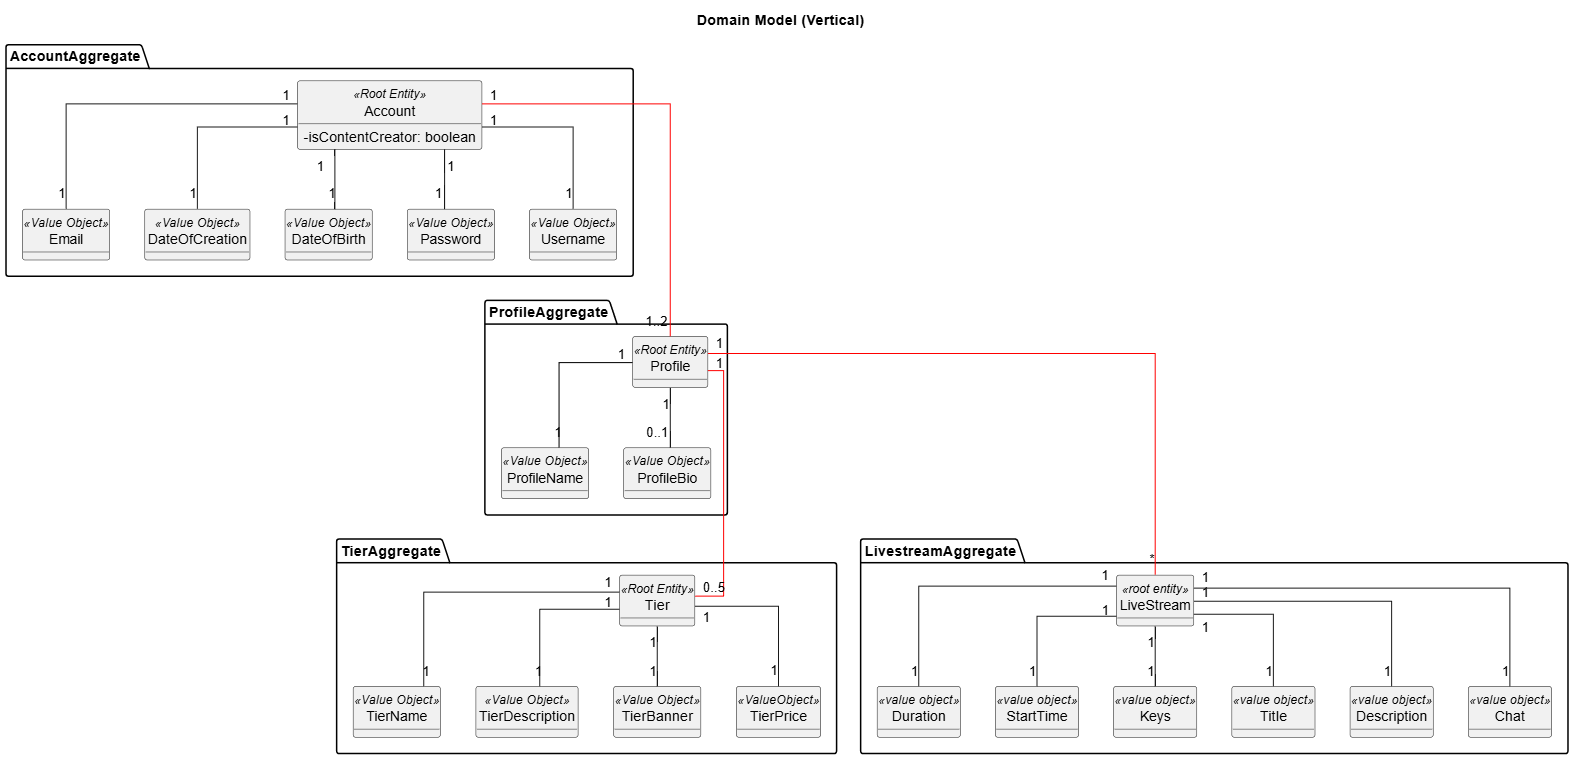
\includegraphics[width=1\textwidth]{frontmatter/assets/design/DomainModel.png}
\caption{Modelo de Dominio - Streaming}
\label{fig-domainModel}
\end{figure}

A solução é composta por quatro agregados principais: \textit{Account}, \textit{Profile}, \textit{Tier}, \textit{Livestream}. Cada agregado define e representa uma área funcional do domínio, composta pela sua entidade e pelos seus objetos.

As ligações entre agregados são as seguintes:

O agregado \textit{Account} é responsável pela integridade dos utilizadores, composta por identificadores, \textit{email} e \textit{username}, e por objetos que servem apenas para conformidades e para fornecer uma melhor experiência ao utilizador. O agregado \textit{Account} liga-se ao agregado \textit{profile} numa ligação de um para muitos, mas no caso do domínio a sua multiplicidade será de uma para um ou dois.

O agregado \textit{Profile} representa a identidade visual do utilizador na aplicação. Um utilizador pode ter um ou dois perfis, sendo o primeiro publico e com acesso a todos os utilizadores e o segundo só permitido a utilizadores que tenham o escalão definido pelo utilizador. Após a criação do perfil privado o sistema permite ao utilizador criar o seu ambiente de transmissão e o seu ambiente de escalões.

O agregado \textit{Tier} modela os níveis de acesso e benefícios por perfil. Contém \textit{TierName}, \textit{TierDescription}, \textit{TierBanner} e \textit{TierPrice}, impondo as seguintes invariantes: no máximo cinco \textit{tiers} por \textit{Profile}.

O agregado \textit{LiveStream} encapsula o ciclo de vida de uma transmissão em direto, incluindo \textit{Title}, \textit{Description}, \textit{StartTime}, \textit{Duration}, \textit{Keys} e \textit{Chat}. Este agregado é dependente da criação de um perfil privado.

\section{Requisitos Funcionais e não funcionais}

Para continuar o desenho da solução, foi necessário declarar e especificar os requisitos que a aplicação deve cumprir. Os requisitos apresentados foram definidos nas \textit{daily meetings} com a equipa e validados pelo supervisor.

Nesta secção vão ser apresentados dois tipos de requisitos:

\begin{itemize}
    \item Requisitos funcionais
    \item Requisitos não funcionais
\end{itemize}

\subsection{Requisitos Funcionais}

Um requisito funcional clarifica no âmbito funcional, as restrições e os critérios de qualidade a que a aplicação deve obedecer.

"Functional requirements capture the intended behavior of the system. This behavior may be expressed as
services, tasks or functions the system is required to perform."\cite{MalanBredemeyer2001FuncReqUseCases}


\begin{table}[H]
\small
\caption{Requisitos Funcionais}
\label{tab:req-funcionais}
\begin{center}
\begin{tabular}{|c|p{13cm}|}
\hline
\textbf{Nº} & \textbf{Descrição do Requisito} \\ \hline
RF01 & O sistema deve permitir iniciar uma transmissão de forma intuitiva e rápida. \\ \hline
RF02 & O sistema deve permitir encerrar uma transmissão de forma intuitiva e rápida. \\ \hline
RF03 & O sistema deve bloquear o acesso a visualizadores que não possuam o \textit{tier} adequado para visualizar uma transmissão. \\ \hline
RF04 & O sistema deve permitir ao criador o controlo do título, descrição, câmara, microfone e cena. \\ \hline
RF05 & O sistema deve confirmar que o criador tem perfil privado para criar uma transmissão em direto. \\ \hline
RF06 & O sistema deve permitir que o criador personalize o menu interativo da transmissão. \\ \hline
RF07 & O sistema deve usar o serviço de \textit{streaming} da AWS para melhor monitorização. \\ \hline
RF08 & O sistema deve permitir interação entre criador e visualizadores através de um \textit{chat} em tempo real. \\ \hline
\end{tabular}
\end{center}
\end{table}


\subsection{Requisitos Não Funcionais}

Nesta secção estabelece-se o enquadramento dos requisitos não funcionais e do modelo FURPS+ ligando-os aos requisitos funcionais.

"Non-functional requirements help deliver a positive user experience and
ensure that product performs to the standards set by stakeholders, clients, and customers."\cite{Rashid2024FURPSMoSCoW}




\subsubsection{FURPS+}

O modelo \gls{FURPS+}, serve para classificar em atributos de qualidade um softwate \cite{Rashid2024FURPSMoSCoW}:

\begin{itemize}
  \item \textit{Functionality}: Especificações funcionais que, em geral, representam as principais funcionalidades da solução.
  \item \textit{Usability}: Considera aspetos da interface do utilizador, como estética e consistência.
  \item \textit{Reliability}:Característica que está associada à inoperabilidade, recuperação em caso de falhas e integridade da aplicação.
  \item \textit{Performance}: Refere-se aos tempos de resposta, eficiência, escalabilidade e utilização
dos recursos da aplicação.
  \item \textit{Supportability}: Característica relacionada com testes, compatibilidade e adaptabilidade da aplicação. 
\end{itemize}

No sistema:

\noindent\textbf{Functionality}
\begin{itemize}
  \item Iniciar e terminar transmissão em dois cliques (RF01/RF02)
  \item Autorização por escalão antes de emitir a transmissão (RF03)
  \item Bloquear criação da transmissão se o perfil não cumprir os critérios. (RF03/RF05)
  \item Controlos do criador (título, descrição, câmara, microfone, cena) com pré-visualização. (RF04)
  \item Menu interativo configurável pelo criador com descrição, preço e visibilidade. (RF06)
  \item Garantir interatividade pelo \textit{chat} (RF08)
\end{itemize}

\noindent\textbf{Usability}
\begin{itemize}
  \item A interface deve ser intuitiva e consistente, permitindo ao utilizador navegar facilmente entre funcionalidades.
  \item O sistema deve apresentar mensagens de erro e \textit{feedback} claro sobre o estado das operações.
\end{itemize}

\noindent\textbf{Reliability}
\begin{itemize}
  \item As validações na criação e atualização de dados devem garantir a integridade da aplicação, evitando operações não autorizadas.
\end{itemize}

\noindent\textbf{Performance}
\begin{itemize}
  \item O sistema deve permitir uma latência minima de acordo com a capacidade de rede de cada utilizador.
  \item Não deve haver perda significativa de qualidade durante a transmissão.
\end{itemize}

\noindent\textbf{Supportability}
\begin{itemize}
  \item A solução deve ser modular, permitindo que os componentes sejam alterados, testados e mantidos de forma independente.
  \item A solução deve permitir que os utilizadores utilizem diversos navegadores.
\end{itemize}

\noindent\textbf{+ Scalability}
\begin{itemize}
  \item A estrutura modular deve permitir a integração com novas áreas de negócio sem comprometer o desempenho do sistema e a experiência do utilizador.
\end{itemize}




\section{Casos de Uso}

Na solução, foram considerados dois atores que fazem parte do sistema, o criador e o visualizador, os casos de uso foram divididos conforme as responsabilidades de cada ator.

Para melhor compreensão e legibilidade do documento os diagramas de caso de uso passaram para os anexos.\ref{AppendixUseCaseCreatorConfiguration}  \ref{AppendixUseCaseCreatorInteraction}

Na Tabela~\ref{tab:uc-creator} estão apresentados os casos de uso do criador:

% Tabela — Casos de uso do ator Creator
\begin{table}[H]
\centering
\caption{Casos de uso do ator \textit{Creator} \ref{AppendixUseCaseCreatorConfiguration} \& \ref{AppendixUseCaseCreatorInteraction}}
\label{tab:uc-creator}
\small
\begin{tabular}{|c|p{11cm}|}
\hline
\textbf{ID} & \textbf{Caso de uso} \\ \hline
C1  & Definir um titulo para a minha transmissão \\ \hline
C2  & Definir uma descrição para a minha transmissão \\ \hline
C3  & Pre-Visualizar a minha transmissão \\ \hline
C4  & Visualizar a minha transmissão \\ \hline
C5  & Iniciar a minha transmissão \\ \hline
C6  & Definir a minha câmara \\ \hline
C7  & Definir o meu microfone \\ \hline
C8  & Silenciar o meu microfone \\ \hline
C9  & Ocultar a minha câmara \\ \hline
C10 & Terminar a minha transmissão \\ \hline
C11 & Visualizar o chat da minha transmissão \\ \hline
C12 & Interagir com o chat da minha transmissão \\ \hline
C13 & Criar um menu interativo para a minha transmissão \\ \hline
C14 & Definir tiers para a minha transmissão \\ \hline
\end{tabular}
\end{table}

Na Tabela~\ref{tab:uc-viewer} estão apresentados os casos de uso do visualizador:
% Tabela — Casos de uso do ator Viewer
\begin{table}[H]
\centering
\caption{Casos de uso do ator \textit{Viewer} \ref{AppendixUseCaseViewer}}
\label{tab:uc-viewer}
\small
\begin{tabular}{|c|p{11cm}|}
\hline
\textbf{ID} & \textbf{Caso de uso} \\ \hline
V1 & Visualizar a transmissão de um Creator \\ \hline
V2 & Interagir com o chat da transmissão \\ \hline
V3 & Controlar a visualização [play,mute,fullscreen,return to Live] \\ \hline
V4 & Definir a qualidade da transmissão \\ \hline
\end{tabular}
\end{table}



\section{Desenho} 

Nesta secção, a solução foi desenhada através do modelo C4, contempla diferentes vistas, o modelo de dados e a relação entre as tabelas. Por fim, foram desenhados os \gls{SSD} para completar o resto da arquitetura.

\subsection{Modelo C4}

O modelo C4, apresentado por Simon Brown no vídeo \cite{Brown2019C4Video} propõe uma abordagem hierárquica e incremental para comunicar arquiteturas de software, o modelo divise-se em quatro camadas:

\begin{itemize}
    \item \textit{System Context} - O sistema mais os utilizadores e as suas dependências.
    \item \textit{Containers} - A forma global da arquitetura e as escolhas tecnológicas.
    \item \textit{Components} - Os componentes lógicos e as respetivas interações dentro do \textit{container}.
    \item \textit{Code}- Detalhes de implementação.
\end{itemize}

\subsection{Nível 1}

Na Figura~\ref{fig-logicView1} é mostrado a vista mais simples do sistema, apenas com o componente central e os serviços externos ao mesmo.

\begin{figure}[H]
\centering
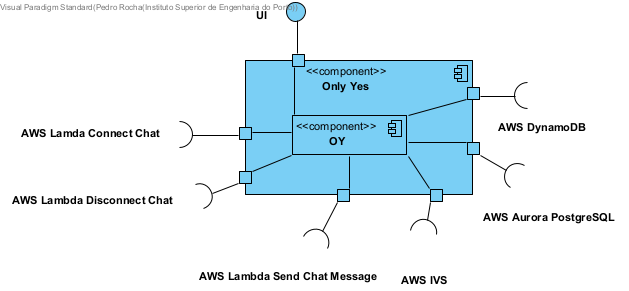
\includegraphics[width=1\textwidth]{frontmatter/assets/design/LogicViewNV1.png}
\caption{Vista Lógica do Sistema - Nível 1}
\label{fig-logicView1}
\end{figure}

O sistema disponibiliza uma interface a ser consumida pelo utilizador e consome outros serviços, descritos na Tabela~\ref{tab:systemServices} :

\begin{table}[H]
\centering
\caption{Serviços disponibilizados para o consumo do sistema}
\label{tab:systemServices}
\small
\begin{tabular}{|c|p{9cm}|}
\hline
\textbf{Serviço} & \textbf{Descrição} \\ \hline
AWS Lambda Connect Chat & Função \textit{serverless} que permite ao utilizador juntar-se a \textit{webSocket} para receber e enviar mensagens em tempo real. \\ \hline
AWS Lambda Disconect Chat & Função \textit{serverless} que permite ao utilizador sair da \textit{webSocket} e da sala de transmissão.  \\ \hline
AWS Lambda Send Chat Message &  Função \textit{serverless} que permite ao utilizador enviar mensagens para o \textit{chat} da sala de transmissão. \\ \hline
AWS IVS &  Serviço gerido pela AWS que cria os canais de transmissão e as credenciais únicas de cada criador.\\ \hline
AWS Aurora PostgreSQL & Base de dados SQL gerida pela AWS.\\ \hline
AWS DynamoDB & Base de dados NoSQL gerida pela AWS \\ \hline
\end{tabular}
\end{table}
    
\subsection{Nível 2}

A Figura~\ref{fig-logicView2} apresenta-se uma vista que divide o componente principal no \textit{front-end} e no \textit{back-end}, cada um com as suas ligações aos respetivos serviços.

\begin{figure}[H]
\centering
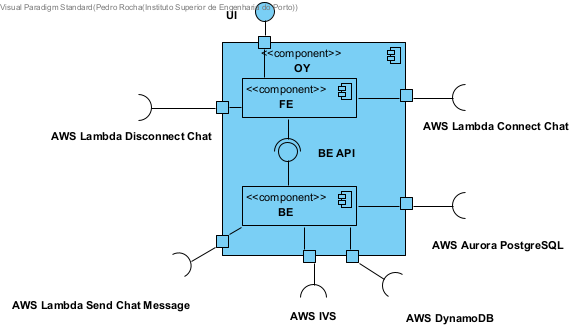
\includegraphics[width=1\textwidth]{frontmatter/assets/design/LogivViewNV2.png}
\caption{Vista Lógica do Sistema - Nível 2}
\label{fig-logicView2}
\end{figure}

O componente BE(\textit{back-end}) proporciona uma APIREST que o componente FE(\textit{front-end}) consome.


\subsection{Nível 3}

No nível três, deste modelo, começa-se por apresentar a vista lógica do \textit{back-end}.

\begin{figure}[H]
\centering
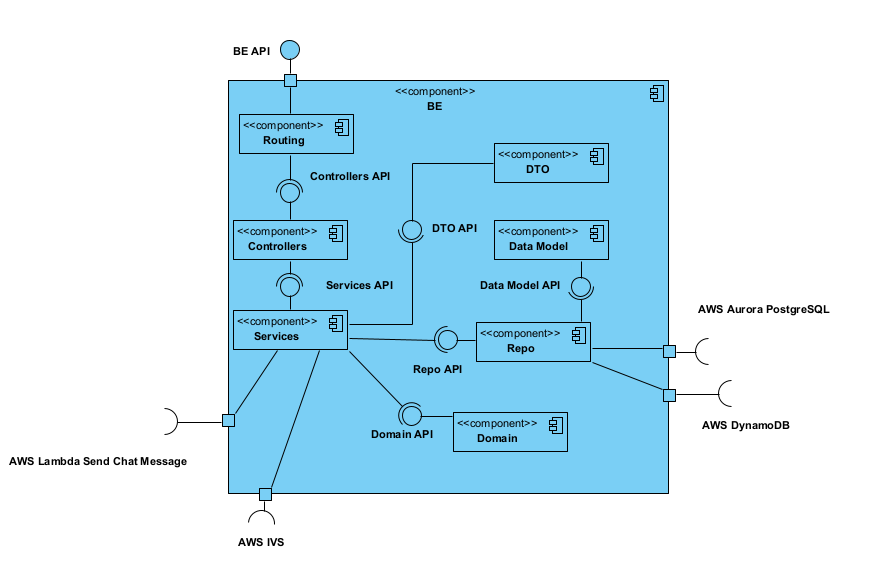
\includegraphics[width=1\textwidth]{frontmatter/assets/design/BELogicViewNV3.png}
\caption{Vista Lógica do \textit{Back-End} - Nível 3}
\label{fig-BeLogivView}
\end{figure}

Pela Figura~\ref{fig-BeLogivView} conseguimos observar as boas práticas do desenvolvimento de software, especificamente a separação de responsabilidades.

Os componentes desta vista são:

\begin{itemize}
    \item \textbf{Routing} - Definem os \textit{endpoints} da aplicação que o \textit{front-ent} pode usar, e redireciona para os \textit{Controllers}.
    \item \textbf{Controllers} - Estes recebem os pedidos e redirecionam para os diversos serviços da aplicação.
    \item \textbf{Services} - Contém a lógica da aplicação, servem de ponte para os repositórios.
    \item \textbf{\gls{DTO}} - Este componente define o que tranferir de cada objeto pela aplicação.
    \item \textbf{Data Model} - Modelo de ligação ás bases de dados.
    \item \textbf{Repo} - Responsável pela persistência dos dados.
    \item \textbf{Domain} - Núcleo da aplicação, trazem o negócio para o código. 
\end{itemize}

Também é possível perceber que o \textit{back-end} integra na totalidade com as bases de dados e com os serviços que precisam de mais segurança como o IVS e a função de enviar mensagem pelo \textit{chat}

Neste nível, também é apresentado a vista de implementação:

\begin{figure}[H]
\centering
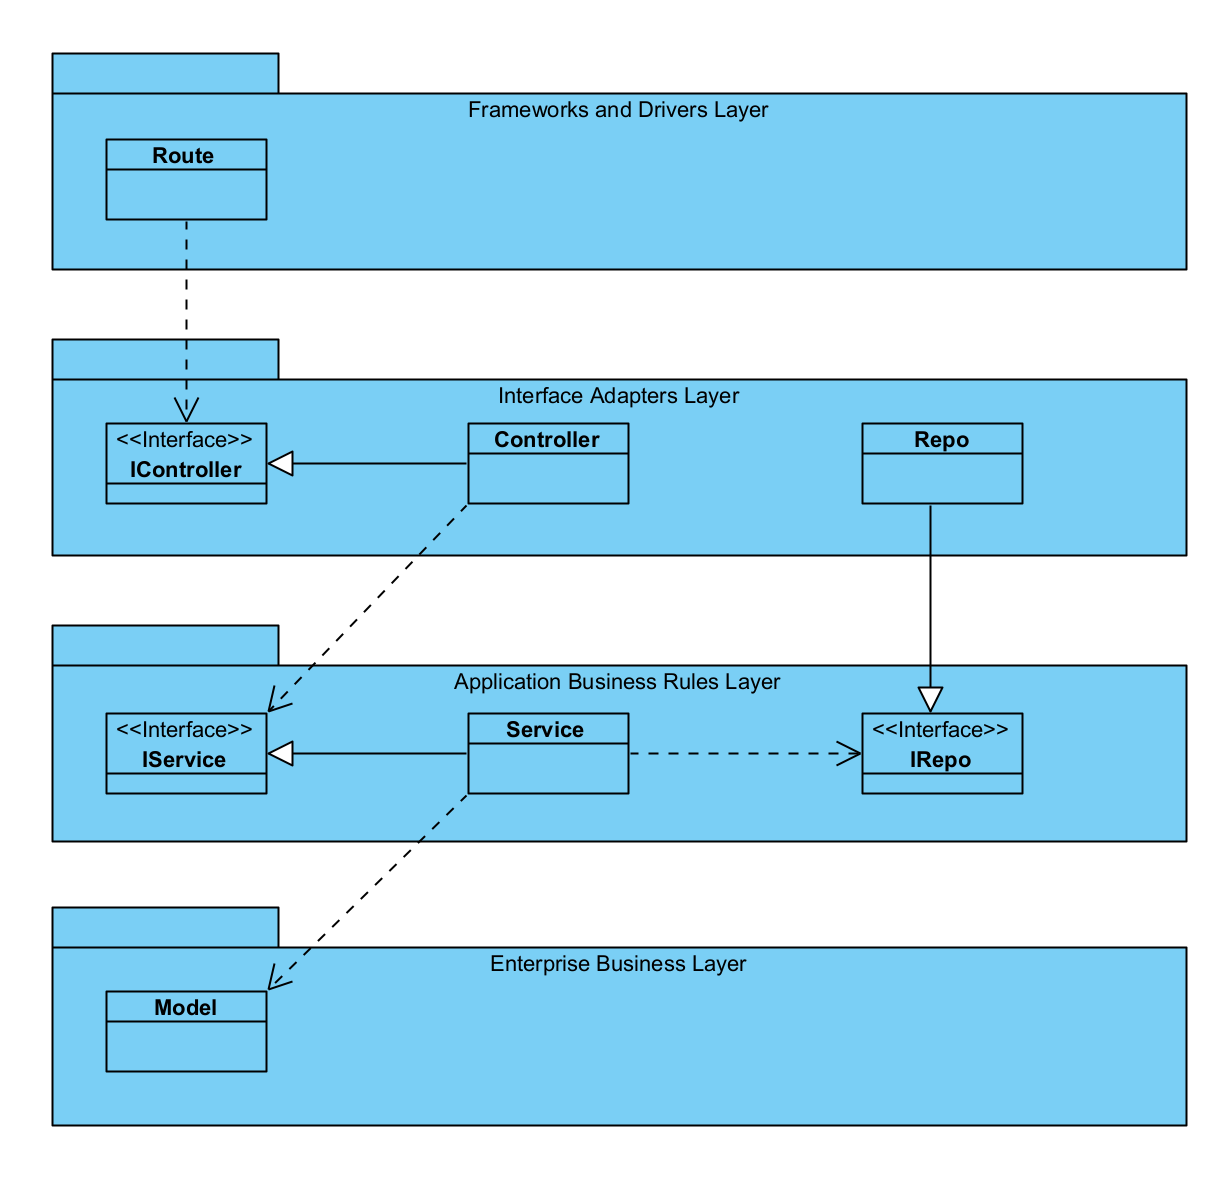
\includegraphics[width=1\textwidth]{frontmatter/assets/design/VistaDeImplementação.png}
\caption{Vista de implementação}
\label{fig-VistaImpl}
\end{figure}

Nesta vista evidenciam-se camadas com dependências orientadas do exterior para o interior que terminam com interfaces. Esta em conformidade com o \gls{DIP}.
Assim, camadas internas não referenciam diretamente implementações externas, por exemplo: \texttt{Service} depende de \texttt{IRepo} e não de \texttt{Repo}.

A vista seguinte incide sobre o componente \textit{front-end} da solução.

\begin{figure}[H]
\centering
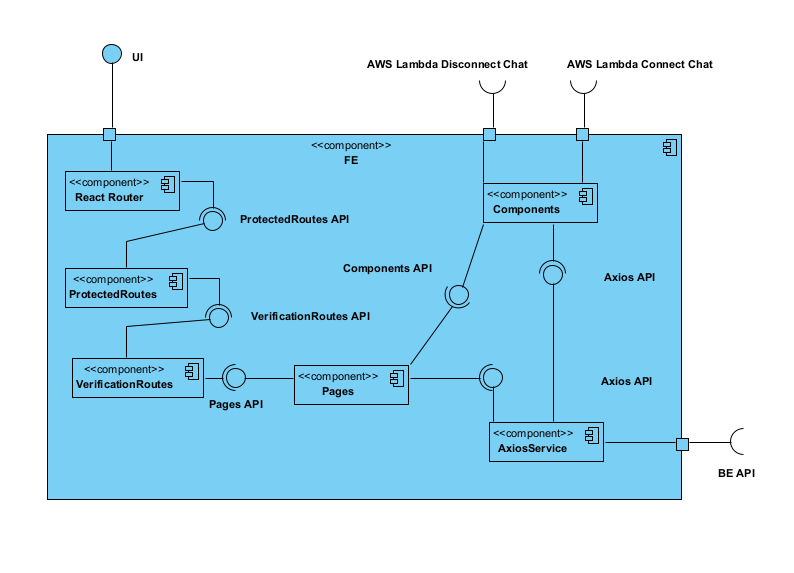
\includegraphics[width=1\textwidth]{frontmatter/assets/design/FELogivViewNV3.png}
\caption{Vista Lógica Nível 3 - \textit{Front-End}}
\label{fig-logicViewFEN3}
\end{figure}

A Figura~\ref{fig-logicViewFEN3} apresenta os seguintes componentes:

\begin{itemize}
    \item \textbf{React Router} - Gere o sistema de navegação da aplicação
    \item \textbf{Protected Route} - verifica as permissões de acesso, no caso da solução verifica se o utilizador está autenticado. 
    \item \textbf{Verification Route} - Aumenta a barreira de segurança, pois verifica se o utilizador tem permissão para assistir ou criar uma transmissão. 
    \item \textbf{Pages} - Conjunto das páginas da aplicação.
    \item \textbf{Components} - Biblioteca de componentes reutilizáveis pelas páginas ou por outros componentes.
    \item \textbf{Axios Service} - Responsável pela comunicação com o \textit{back-end} 
\end{itemize}

\subsection{Vista Física}

Como toda a infraestrutura da solução reside na \gls{AWS}, nesta fase de desenho foi necessário aplicar os conhecimentos obtidos na formação.

\begin{figure}[H]
\centering
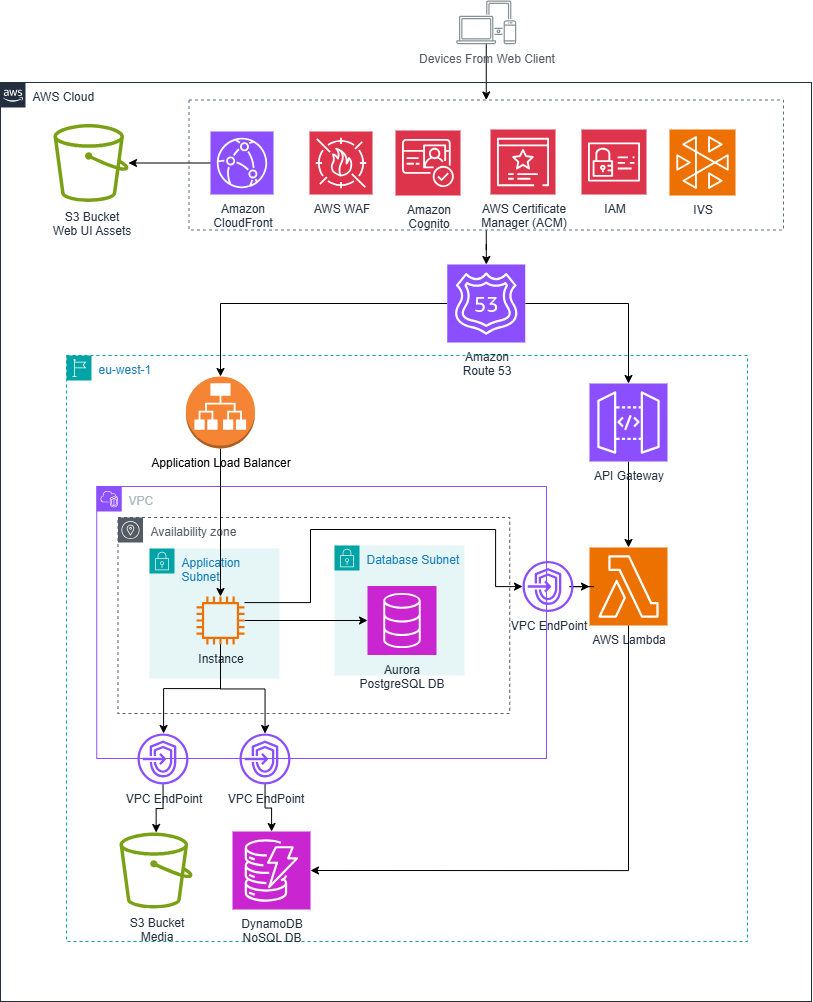
\includegraphics[width=1\textwidth]{frontmatter/assets/design/vf.png}
\caption{Vista física - Infraestrutura AWS}
\label{fig-vistaFisica}
\end{figure}

Na Figura~\ref{fig-vistaFisica} são apresentados os seguintes serviços:
\begin{table}[H]
\centering
\small
\caption{Serviços AWS e respetivo papel na solução}
\label{tab:aws-servicos}
\begin{tabular}{|p{4.3cm}|p{9.7cm}|}
\hline
\textbf{Serviço} & \textbf{Descrição} \\ \hline
Amazon Route 53 & Resolução de nomes do domínio da aplicação\\ \hline
Amazon CloudFront & Distribuição de conteúdos estáticos do S3\\ \hline
Amazon S3 (UI) & Contêm os conteúdos estáticos do \textit{front-end} \\ \hline
Amazon S3 (Media) & Repositório de conteúdos multimédia (vídeos/fotos) . \\ \hline
AWS \gls{WAF} & Controlo do tráfego na aplicação\\ \hline
\gls{ACM} & Emite certificados \gls{SSL} para a aplicação. \\ \hline
\gls{ALB} & Distribui o tráfego de pedidos para diversas instâncias da aplicação. \\ \hline
Amazon \gls{VPC} & Isola a rede da aplicação com, \textit{subnets}, \textit{security groups} e \textit{routing table}. \\ \hline
VPC Endpoints & Permite aceder a serviços fora da VPC. \\ \hline
Amazon API Gateway & Expõem \textit{enpoints} para o acesso as funções Lambda. \\ \hline
AWS Lambda & Função \textit{serverless} que consegue fazer \textit{build} de codigo independente. \\ \hline
Amazon Aurora PostgreSQL & Base de dados SQL \\ \hline
Amazon DynamoDB & Base de dados NoSQL\\ \hline
AWS \gls{IVS} & Serviço gerido pela AWS que cria os canais de transmissão e as credenciais únicas de cada criador. \\ \hline
AWS \gls{IAM} & Controla o acesso da aplicação. \\ \hline
\end{tabular}
\end{table}


Passando para uma explicação mais estruturada, em primeira instância, os dispositivos dos utilizadores acedem à aplicação, cujo nome é resolvido no \textbf{Amazon Route 53}.

O conteúdo do \textit{front-ent} é alojados pelo \textbf{Amazon CloudFront} a partir de \textbf{Amazon S3}, com proteção \textbf{AWS WAF} e para segurança através do protocolo \gls{TLS} via \textbf{Amazon Certificate Manager}.

As chamadas do \textit{front-end} seguem dois percursos:
\begin{itemize}
    \item Através de um \textbf{Application Load Balancer} para a APIREST do \textit{back-end}.
    \item Através \textit{API Gateway} para funções \textit{AWS Lambda} quando adequado.
\end{itemize}

A persistência é feita por \textbf{Amazon Aurora PostgreSQL} (base de dados SQL), \textbf{DynamoDB} (base de dados NoSQL) e \textbf{S3} (para objetos como imagens e vídeos).

O \textbf{AWS IVS} suporta as transmissões em direto e o \textbf{IAM} controla o acesso aos recursos da infraestrutura.

Com estes serviços a solução garante escalabilidade, disponibilidade e segurança.


\subsection{Modelo de Dados}

Após a descrição do sistema, o modelo de dados foi desenhado para ajudar na compreensão do domínio e na construção das bases de dados.

\begin{figure}[H]
\centering
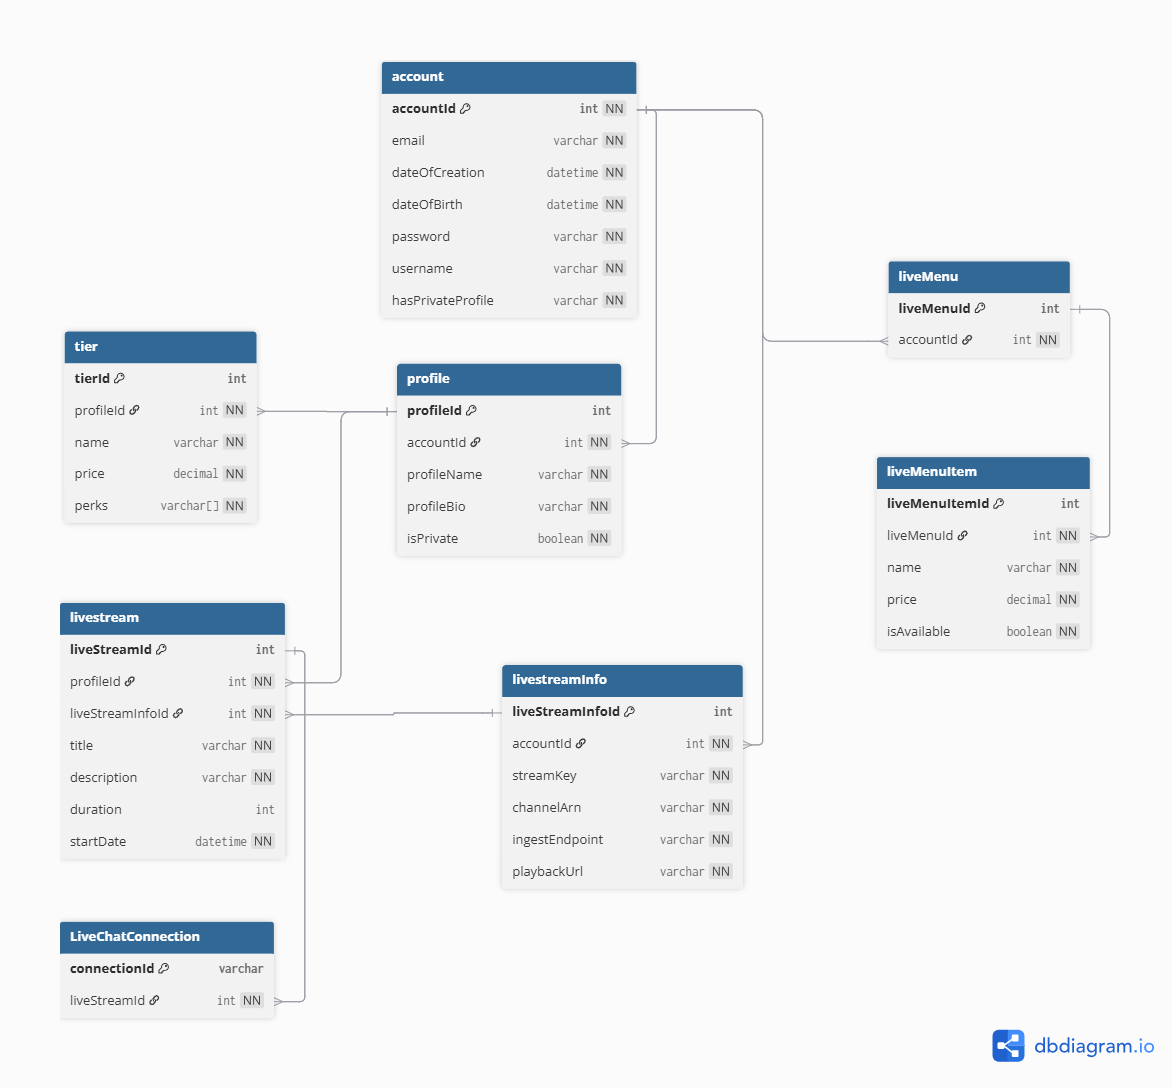
\includegraphics[width=1\textwidth]{frontmatter/assets/design/modeloDados.png}
\caption{Modelo de Dados}
\label{fig-modeloDados}
\end{figure}

Na Figura~\ref{fig-modeloDados}, está representado o modelo de dados adotado para a criação do dominio do código.

Adotou-se um modelo híbrido, que combina a base de dados relacional (PostgreSQL) e a base de dados não-relacional (DynamoDB).

A camada relacional preserva a integridade do modelo, onde são garantidas as regras de negocio e transações \gls{ACID}.

A camada não-relacional serve para objetos de grande leitura e editáveis.

\textbf{SQL}
\begin{itemize}
\item \textbf{Account}: accountId, email, dateOfCreation, dateOfBirth, password, username, hasPrivateProfile.
\item \textbf{Profile}: profileId, accountId, isPrivate.
\item \textbf{Tier}: tierId, profileId.
\item \textbf{LiveStreamInfo}: liveStreamInfoId, accountId, streamKey, channelArn, ingestEndpoint, playbackUrl.
\item \textbf{LiveStream}: liveStreamId, profileId, liveStreamInfoId.
\item \textbf{LiveMenu}: accountId, liveMenuId.
\item \textbf{LiveMenuItem}: liveMenuItemId, liveMenuId, isAvailable.
\end{itemize}

\textbf{DynamoDB}
\begin{itemize}
\item \textbf{Profile}: profileId, name, bio.
\item \textbf{Tier}: tierId, name, price, perks.
\item \textbf{LiveStream}: liveStreamid, title, description, duration, startDate.
\item \textbf{LiveMenuItem}: liveMenuItemId, name, price.
\item \textbf{LiveChatConnection} : connectionId, liveStreamId.
\end{itemize}

Como as transmissões não serão gravadas, não houve a necessidade de fazer um modelo de dados para o \textit{chat}.

\subsection{Diagramas de sequência dos casos de uso}


Nesta secção apresentam-se diagramas que explicam como cada caso de uso é executado ao nível das interações entre o ator e o sistema.

Para privilegiar a legibilidade e reduzir a poluição visual, os diagramas incluídos no corpo do texto encontram-se deliberadamente simplificados, representando apenas dois participantes: \textit{Ator} e \textit{Sistema}. O participante \textit{Sistema} agrega, de forma abstrata, os componentes internos e respetivos fluxos.

As versões completas e detalhadas dos diagramas estão na secção dos anexos:

\begin{itemize}
    \item Diagrama de Sequência do \textit{back-end}~\ref{fig-ssdBEFULL}.
    \item Diagrama de Sequência do \textit{front-end}~\ref{fig-ssdFEFULL}.
    \item Diagrama de Sequência do sistema~\ref{fig-ssdFULL}.
\end{itemize}

\subsubsection{Casos de Uso \textbf{C1} \& \textbf{C2}}

O diagrama de sequência~\ref{fig-SSDTITULODESC}, cobre os casos de uso que descrevem a configuração inicial do criador para criar um ambiente de transmissão. Descreve as validações necessárias para criar o título e a descrição, e inclui a persistência de dados.

\begin{figure}[H]
\centering
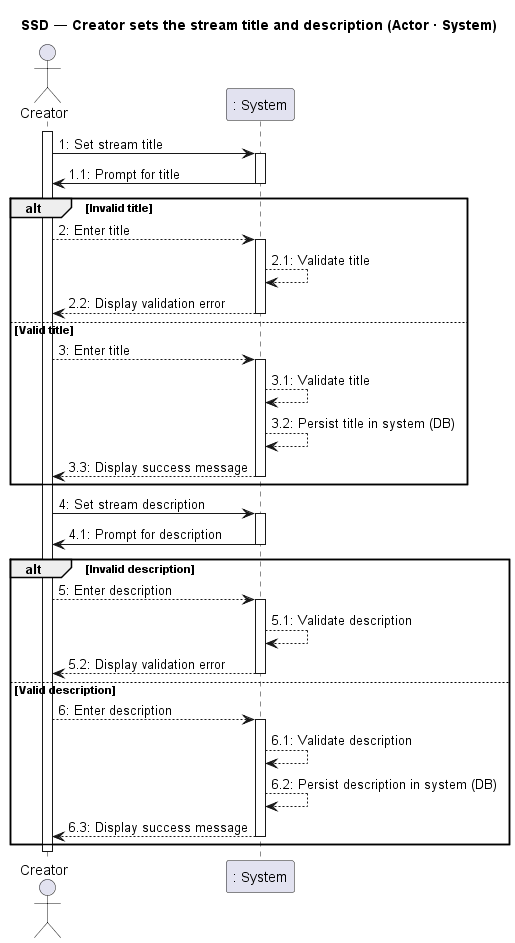
\includegraphics[width=\textwidth,height=0.8\textheight,keepaspectratio]{frontmatter/assets/ssd/SSD-CR-002.png}
\caption{Diagrama de sequência do sistema para criar título e descrição da transmissão.}
\label{fig-SSDTITULODESC}
\end{figure}

\subsubsection{Casos de Uso \textbf{C6} \& \textbf{C7} \& \textbf{C3}}

O diagrama de sequência~\ref{fig-SSD-CR-CAM-MIC}, mostra a configuração da câmara e do microfone, através do \textit{MediaStream} referido anteriormente no capítulo \ref{chap:EA}, com permissões pedidas pelo \textit{browser}, ao utilizador e uma \textit{preview} da transmissão.  

\begin{figure}[H]
\centering
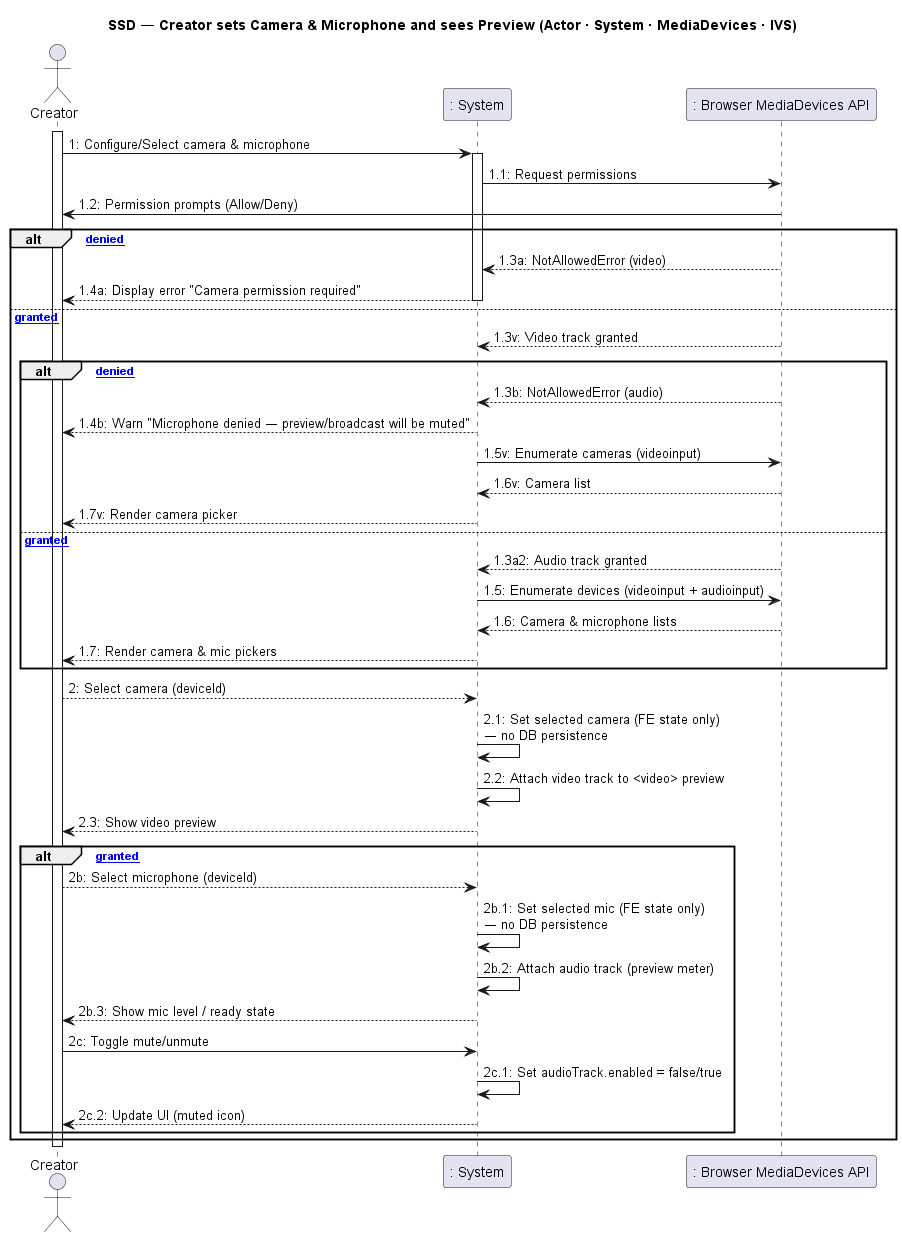
\includegraphics[width=\textwidth,height=0.8\textheight,keepaspectratio]{frontmatter/assets/ssd/SSD-CR-CAM-MIC.png}
\caption{Diagrama de sequência do sistema para configurar câmara e microfone (ativação, permissões e teste).}
\label{fig-SSD-CR-CAM-MIC}
\end{figure}

\subsubsection{Casos de Uso \textbf{C8} \& \textbf{C9}}

O diagrama de sequência~\ref{fig-SSD-CR-CAM-MIC-OFF}, descreve a ação de desativar e reativar o microfone e desligar a câmara. Ambas as açães geram notificações ao utilizador melhorando a sua experiência.

\begin{figure}[H]
\centering
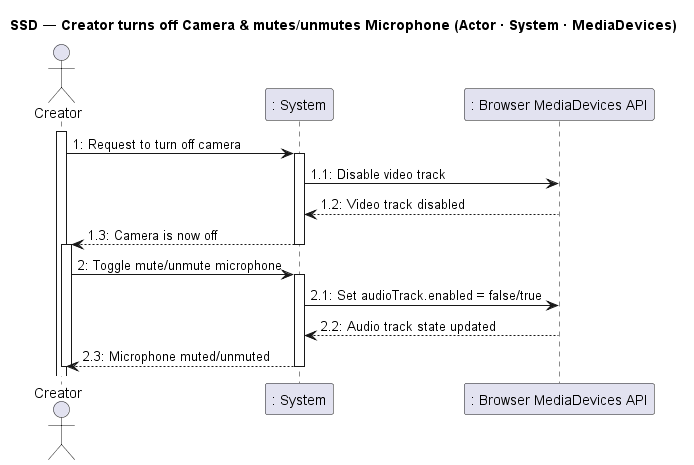
\includegraphics[width=\textwidth,height=0.6\textheight,keepaspectratio]{frontmatter/assets/ssd/SSD-CR-CAM-MIC-OFF.png}
\caption{Diagrama de sequência do sistema para desativar/reativar câmara e microfone durante a transmissão.}
\label{fig-SSD-CR-CAM-MIC-OFF}
\end{figure}

\subsubsection{Casos de Uso \textbf{C5} \& \textbf{C10}}

O diagrama de sequência~\ref{fig-SSD-CR-START-STREAM}, simplifica e descreve a ação de começar uma transmissão, o sistema verifica todos os requisitos antes de criar a \textit{stream}.

\begin{figure}[H]
\centering
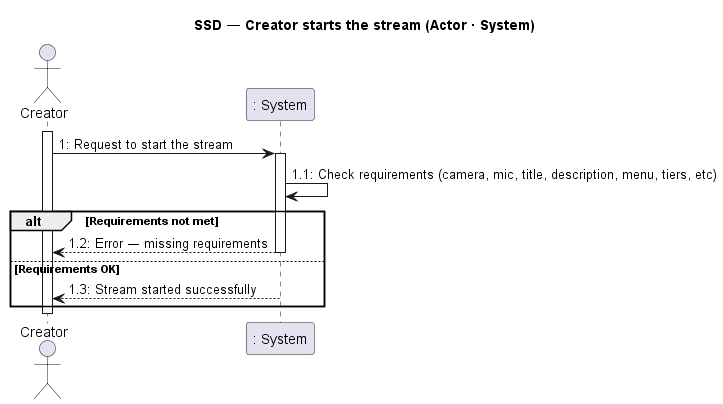
\includegraphics[width=\textwidth,height=0.8\textheight,keepaspectratio]{frontmatter/assets/ssd/SSD-CR-START-STREAM.png}
\caption{Diagrama de sequência do sistema para iniciar a transmissão (\textit{start stream}).}
\label{fig-SSD-CR-START-STREAM}
\end{figure}

O diagrama de sequência~\ref{fig-SSD-CR-STOP-STREAM}, descreve a simplicidade de acabar uma transmissão.

\begin{figure}[H]
\centering
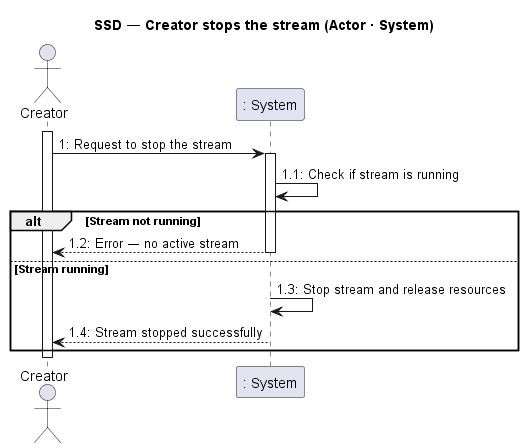
\includegraphics[width=\textwidth,height=0.6\textheight,keepaspectratio]{frontmatter/assets/ssd/SSD-CR-STOP-STREAM.png}
\caption{Diagrama de sequência do sistema para terminar a transmissão (\textit{stop stream}).}
\label{fig-SSD-CR-STOP-STREAM}
\end{figure}

\subsubsection{Caso de Uso \textbf{C11}}

O diagrama de sequência~\ref{fig-SSD-CR-CHAT-VIEW}, descreve como o criador entra na sua própria página de \textit{stream}, e por \textit{web-socket}, liga-se a sala de \textit{chat}. Após ligar-se fica capaz de receber mensagens em tempo real por outros utilizadores que estejam na mesma sala.

\begin{figure}[H]
\centering
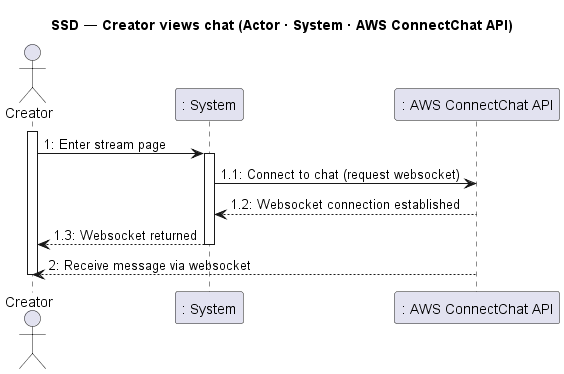
\includegraphics[width=\textwidth,height=0.6\textheight,keepaspectratio]{frontmatter/assets/ssd/SSD-CR-CHAT-VIEW.png}
\caption{Diagrama de sequência do sistema para visualização do chat pelo criador.}
\label{fig-SSD-CR-CHAT-VIEW}
\end{figure}

\subsubsection{Caso de Uso \textbf{C12}}

O diagrama de sequência~\ref{fig-SSD-CR-CHAT-INTERACT} especifica a interação ativa do criador com o chat: envio de mensagens, respostas, remoção e moderação. Detalham-se confirmações de entrega (\textit{ack}), tratamento de \textit{rate limits}, e feedback visual para estados em envio/erro. Prevê-se ainda a sincronização com serviços anti-spam e logs de auditoria.

\begin{figure}[H]
\centering
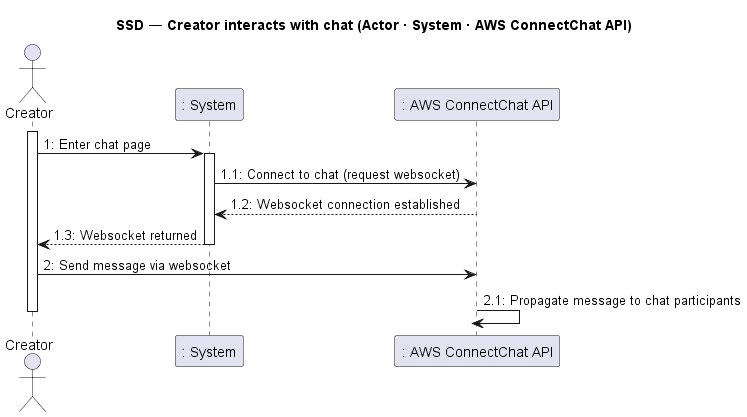
\includegraphics[width=\textwidth,height=0.8\textheight,keepaspectratio]{frontmatter/assets/ssd/SSD-CR-CHAT-INTERACT.png}
\caption{Diagrama de sequência do sistema para interação do criador no chat (envio e moderação).}
\label{fig-SSD-CR-CHAT-INTERACT}
\end{figure}

\subsubsection{Caso de Uso \textbf{C13}}

O diagrama de sequência~\ref{fig-SSD-CR-Menu} foca a gestão e apresentação do \textit{Live Menu} durante a transmissão. Descrevem-se a consulta do catálogo, a atualização de disponibilidade em tempo real e a reflexão imediata das alterações na interface. São também contemplados eventos de sincronização com o backend e métricas de uso.

\begin{figure}[H]
\centering
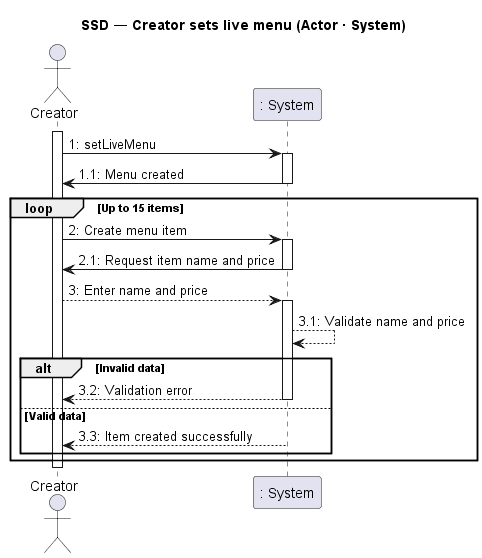
\includegraphics[width=\textwidth,height=0.5\textheight,keepaspectratio]{frontmatter/assets/ssd/SSD-CR-Menu.png}
\caption{Diagrama de sequência do sistema para gestão e apresentação do \textit{Live Menu}.}
\label{fig-SSD-CR-Menu}
\end{figure}

\subsubsection{Caso de Uso \textbf{C14}}

No diagrama de sequência~\ref{fig-SSD-CR-TIER}, aborda-se a gestão de \textit{tiers} de acesso e a sua seleção/atribuição à sessão.

\begin{figure}[H]
\centering
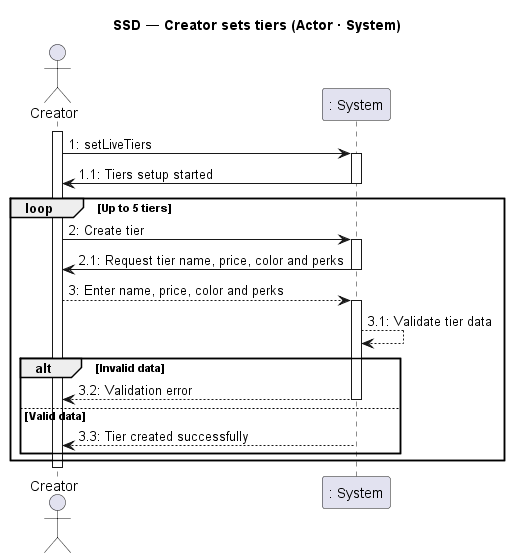
\includegraphics[width=\textwidth,height=0.5\textheight,keepaspectratio]{frontmatter/assets/ssd/SSD-CR-Tier.png}
\caption{Diagrama de sequência do sistema para gestão e seleção de \textit{tiers} de acesso.}
\label{fig-SSD-CR-TIER}
\end{figure}

\subsubsection{Caso de Uso \textbf{V1}}

O diagrama de sequência~\ref{fig-SSD-USER-VIEW-STREAM} descreve a experiência do \textit{viewer} ao iniciar a visualização duma transmissão. Incluem-se a resolução de URL do canal, o estabelecimento da sessão de reprodução, a negociação de qualidade adaptativa e o tratamento de erros iniciais.

\begin{figure}[H]
\centering
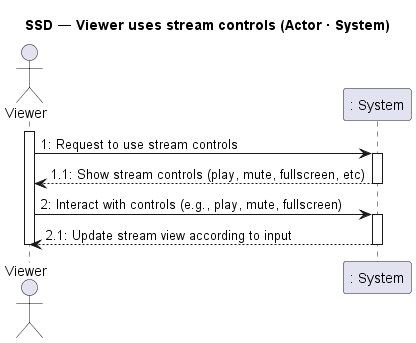
\includegraphics[width=\textwidth,height=0.6\textheight,keepaspectratio]{frontmatter/assets/ssd/SSD-USER-VIEW-STREAM.png}
\caption{Diagrama de sequência do sistema para visualização da transmissão pelo utilizador.}
\label{fig-SSD-USER-VIEW-STREAM}
\end{figure}

\subsubsection{Caso de Uso \textbf{V2}}

O diagrama de sequência~\ref{fig-SSD-USER-CHAT-INTERACT} aborda a interação do utilizador com o \textit{chat} público/privado durante a transmissão. Explicita-se o envio e receção de mensagens em tempo real, limitações de frequência, e \textit{feedback} de entrega. Prevê-se moderação automática e mecanismos de denúncia.

\begin{figure}[H]
\centering
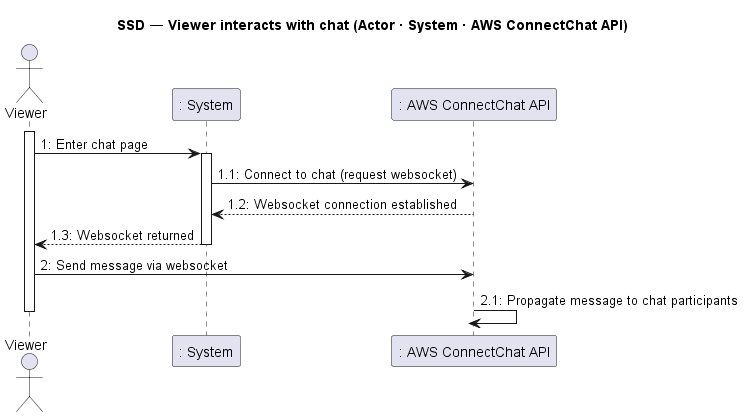
\includegraphics[width=\textwidth,height=0.8\textheight,keepaspectratio]{frontmatter/assets/ssd/SSD-USER-CHAT-INTERACT.png}
\caption{Diagrama de sequência do sistema para interação do utilizador no chat.}
\label{fig-SSD-USER-CHAT-INTERACT}
\end{figure}

\subsubsection{Caso de Uso \textbf{V3}}

No diagrama de sequência~\ref{fig-SSD-USER-VIEW-STREAM-Controlls} detalham-se os controlos de reprodução disponíveis para o utilizador: \textit{play/pause}, volume, \textit{mute}, ecrã inteiro e seleção de qualidade. Define-se a sincronização de estado entre UI e \textit{player}, incluindo atalhos e acessibilidade. Consideram-se ainda indicadores de estado (buffering, erro) e mensagens de orientação.

\begin{figure}[H]
\centering
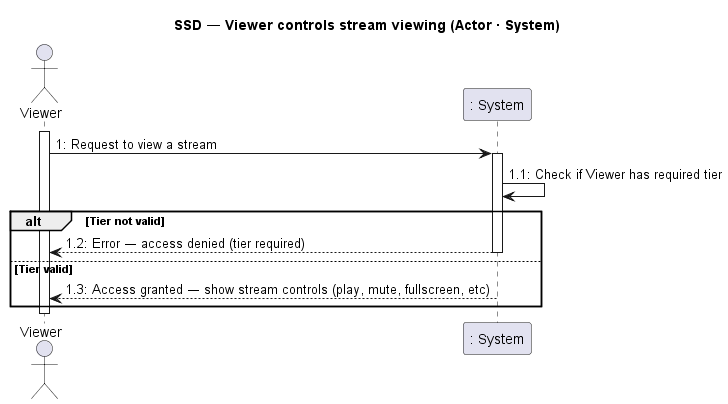
\includegraphics[width=\textwidth,height=0.8\textheight,keepaspectratio]{frontmatter/assets/ssd/SSD-USER-VIEW-STREAM-Controlls.png}
\caption{Diagrama de sequência do sistema para controlos de reprodução da transmissão pelo utilizador.}
\label{fig-SSD-USER-VIEW-STREAM-Controlls}
\end{figure}

\subsection{Alternativas ao \textit{design}}

Consoante o desenvolvimento, foram detetadas alternativas ao desenho da solução, nomeadamente na criação da transmissão. Nos caso de uso apresentados, as configurações como o título de a descrição são persistidos na base de dados antes de iniciar a \textit{live}, por outro lado, poderia ser adequado só persistir nas bases de dado, apenas quando fosse começar uma transmissão.

Em alternativa ao modelo de como as salas de transmissões são feitas, seria prudente criar uma \textit{web-socket}, para a sala em geral, pois para interações em tempo real, não seria necessário criar uma ligação nova a para cada funcionalidade. Exemplificando, quando um visualizador que doar ao criador durante a transmissão, precisa de ser despoletado uma ação de confirmação, e como esse serviço não está ligado a nenhuma "sala", não consegue ser em tempo real. Para resolver este caso foi desenvolvido um "scheduler" no \textit{back-end}, que corre certos métodos em curtos espaços de tempo.

\section{Conclusão}

O capítulo apresentou uma visão completa e coerente do sistema, desde a caracterização do domínio e definição de requisitos até à arquitetura e modelos que os materializam. Clarificaram-se conceitos nucleares (\textit{Account}, \textit{Profile}, \textit{Tier}, \textit{LiveStream}) e respetivas relações, assegurando uma base semântica estável para o desenho técnico. Foram especificados requisitos funcionais (RF01–RF08) e não funcionais, enquadrados no modelo FURPS+, garantindo alinhamento entre necessidades de negócio, usabilidade, fiabilidade, desempenho e suportabilidade.

O desenho arquitetural, estruturado pelo modelo \textit{C4}, evidenciou a separação \textit{FE/BE}, responsabilidades por camadas e dependências internas, culminando numa vista física detalhada em \textit{AWS}

O modelo de dados híbrido (relacional + NoSQL) foi alinhado com o domínio: integridade transacional em Aurora para entidades críticas e projeções e editabilidade em DynamoDB para leitura intensiva, reforçando tanto consistência como performance. Por fim, os diagramas de sequência consolidaram o comportamento por casos de uso.







\label{sec:Des}



